Le domaine 2D occupé par la croûte est noté $\Omega_C$. Les propriétés physiques associées à cette croûte sont : $T_C$ la température, $\rho_C$ la densité, $\lambda_C$ la conductivité thermique, $C_{p,C}$ la capacité thermique, $\Delta {\cal H}^{fus}$ l'enthalpie de fusion et $T_{fus}$ (resp. $T_{sol}$) la température de fusion de la croûte (resp. la température de solidification du corium liquide).


On note $\gamma_{in}$ la partie de la frontière interne du domaine $\Omega_C$ (i.e. côté bain de corium liquide) et $\gamma_{ext}$ la partie de la frontière externe du domaine $\Omega_C$ (i.e. côté cuve), voir figure \ref{fig:crust_figure}. Sur la frontière $\gamma_{in}$, une partie de la croûte est en contact avec le corium liquide, elle est alors soumise à un flux $\phi_{bain}$ provenant du bain de corium liquide. Sur la frontière $\gamma_{ext}$, une condition de température imposée ($T_C=T^{out}$) ou de flux imposé ($\phi=\phi_{out}$) peut être définie.

\begin{figure}[H]
\centering
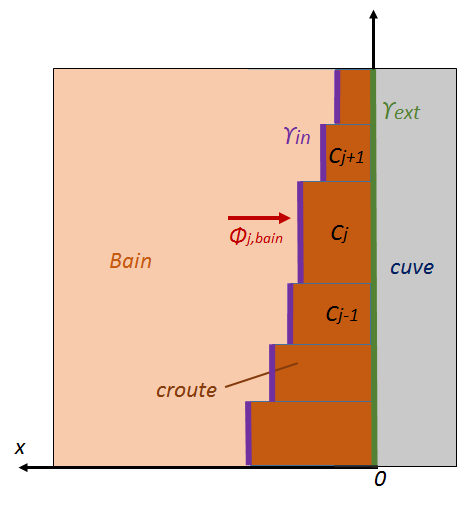
\includegraphics[width=0.4\textwidth]{Figures/crust_figure.png}
\caption{Schéma de la croûte couplée à au bain de corium liquide et de la cuve} \label{fig:crust_figure}
\end{figure}

Le domaine $\Omega_C$ est discrétisé en 1D selon la direction verticale (selon l'axe noté $z$) de la croûte. Le maillage est décrit par $N_{noeuds}$ noeuds. Les $N_{mailles}=N_{noeuds}-1$ mailles rectangulaires correspondantes sont notées $C_j$ pour $1 \leq j\leq N_{mailles}$. Pour chaque maille, la direction horizontale est donnée par l'axe $x$. On note [$x_j^{min}, x_j^{max}$] le domaine occupé par la maille $j$ suivant l'axe $x$ et $S_j$ la surface de la face verticale (i.e. suivant l'axe $z$). A chaque pas de temps, le bain de corium peut changer de configuration (e.g. stratification, baisse ou élévation du niveau du bain). Ainsi, à chaque pas de temps le domaine occupé par la croûte est remaillé à partir d'un pas d'espace de référence en respectant les contraintes suivantes :
\begin{itemize}
    \item une maille ne peut pas être en face de deux couches du bain, ainsi celle-ci ne recevra un flux thermique provenant uniquement d'une seul couche
    \item quelque soit l'épaisseur d'une couche du bain de corium, au moins une maille sera definie en face de cette couche
    \item  Il peut apparaître éventuellement au cours d'un calcul une autre partie de $\gamma_{in}$ située plus haut que le niveau supérieure du bain de corium liquide (e.g. lorsque le niveau du bain baisse, une partie de la croûte ne voit plus le corium liquide). Dans ce cas on considérera une condition adiabatique.
\end{itemize}
A chaque remaillage du domaine occupé par la croûte, une projection des masses et des températures est effectuée sur le nouveau maillage en assurant une conservation en masse et en énergie (voir section \ref{couplage}).

Les quantités moyennes suivantes sont introduites pour $1 \leq j\leq N_{mailles}$ :
\begin{eqnarray}
m_{j}(t) &=& \rho_C  V_j(t) \\
\overline{T}_{j}(t) &=& \frac{1}{V_j(t)} \int_{C_j(t)} T_{j}(x,z,t)\,\mathrm{d}x\, \mathrm{d}z\\
\overline{h}_j(t) &=& \frac{1}{m_j(t)} \int_{C_j(t)} h_j(x,z,t)\,\mathrm{d}x\, \mathrm{d}z\\
\overline{\phi}_{j,in}(t) &=& -\frac{1}{S_j}\int_{\gamma_{in}\cap S_j}\lambda_C \frac{\partial T_{j}}{\partial x}(x=x_j^{min},z,t)\, \mathrm{d}z  \label{eq:phi_j_in}\\
\overline{\phi}_{j,ext}(t) &=& -\frac{1}{S_j}\int_{\gamma_{ext}\cap S_j}\lambda_C \frac{\partial T_{j}}{\partial x} (x=x_j^{max},z,t)\, \mathrm{d}z  \label{eq:phi_j_ext}
\end{eqnarray}
avec $T_{j}$ la température de la maille $j$, $h_j$ l'enthalpie spécifique et $V_j$ le volume de la maille $j$.\\

Le système (\ref{eq:mass})-(\ref{eq:enthalpie}) suivant donne l'évolution des masses et enthalpies spécifiques moyennes pour chaque maille $j$ :

\begin{eqnarray}
\frac{dm_{j}}{dt} &=& - \frac{dm_{j}^\text{fus/sol}}{dt} \label{eq:mass} \\ 
%m_{j} C_{p,C} \frac{d \overline{T}_{j}}{dt} &+& \frac{dm_{j}^\text{fus/sol}}{dt}C_{p,C} \left(T^{fus/sol} - \overline{T}_{j}\right) \\ &=& S_i\left(\overline{\phi}_{j,in} - \overline{\phi}_{j,ext}\right) + \dot{q}^m m_{j}
 \frac{d}{dt}(m_{j}\overline{h}_{j}) + \frac{dm_{j}^\text{fus/sol}}{dt} \overline{h}_{\gamma_{in},j} & = & S_i\left(\overline{\phi}_{j,in} - \overline{\phi}_{j,ext}\right) + \dot{q}^m m_{j} \label{eq:enthalpie}
\end{eqnarray}

où :

\begin{itemize}
 \item $\frac{dm_j^\text{fus/sol}}{dt}$ est le taux de masse ablatée dans le cas d'une fusion de la croûte ou le taux de masse solidifiée dans le cas d'une solidification du corium liquide. Ce taux de masse est positif dans le cas d'une fusion et négatif dans le cas d'une solidification;
 \item $\overline{h}_{\gamma_{in},j}$ représente l'enthalpie spécifique à l’interface $\gamma_{in}$ ;
 \item $\dot{q}^m m$ représente la contribution de la puissance résiduelle ($W$) associée à la puissance résiduelle massique $\dot{q}^m$ ($W/kg$);
\end{itemize}
Dans ce système, la conduction axiale (i.e. suivant l'axe $z$) a été négligée. Il est à noter qu'une option est disponible dans le code pour prendre en compte une approximation numérique de flux thermique axial (\cite{Peybernes2018}). 

Une maille $C_j$ peut être dans trois types "d'état" : soit elle est en fusion, soit en solidification, soit le volume de la maille $C_j$ reste constant. Dans ce dernier cas, on dira par la suite que la maille $C_j$ est en "pure conduction". Par la suite, en considérant que $T_{sol}\leq T_{j,in}\leq T_{fus}$, on supposera qu'une maille $C_j$ doit passer par un état de "pure conduction" pour passer d'un état de fusion à un état de solidification ou inversement.

En fonction de la température de la frontière interne de la croûte $\gamma_{in}$, que l'on note $T_{j,in}$, les fermetures associées au système d'équations précédent sont différentes. Ci-dessous sont listés les différents cas de figure :\\

\begin{itemize}
\item {\it cas d'une pure conduction dans la croûte :}\\
Tant que $T_{j,in}<T_{fus}$, la fusion de la maille de croûte $C_j$ n'a pas commencé :
\begin{eqnarray*}
\frac{dm_j^\text{fus/sol}}{dt} &=& 0.0 \\
\overline{\phi}_{j,in} &=& \phi_{j,bain}
\end{eqnarray*}

\item {\it passage en fusion de la croûte :}\\
Si $T_{j,in}$ atteint la température $T_{fus}$ ($T_{j,in}\ge T_{fus}$), la fusion de la maille $C_j$ commence suivant l'équation de front de fusion suivante :
\begin{eqnarray*}
\Delta \mathcal{H}^{fus} \frac{dm_j^\text{fus/sol}}{dt} &=& S_j\left(\phi_{j,bain} - \overline{\phi}_{j,in}\right) \\
T_{j,in} &=& T^{fus}
\end{eqnarray*}

\item {\it passage en solidification du corium :}\\
Si $T_{j,in}$ atteint la température $T^{sol}$ ($T_{j,in}\le T^sol$), la solidification du corium commence suivant l'équation du front de solidification suivante :
\begin{eqnarray*}
\Delta \mathcal{H}^{fus} \frac{dm_j^\text{fus/sol}}{dt} &=& S_j\left(\phi_{j,bain} - \overline{\phi}_{j,in}\right) \\
T_j^{in} &=& T^{sol}
\end{eqnarray*}

\item {\it passage en conduction pure après un arrêt d'une fusion/solidification :}\\
Lorsque une maille $C_j$ est en fusion ou solidification, si $\frac{dm_i^\text{fus/sol}}{dt}$ s'annule, le front de fusion/solidification s'arrête. Et ainsi la maille $C_j$ devient en "conduction pure" :
\begin{eqnarray*}
\frac{dm_j^\text{fus/sol}}{dt} &=& 0.0 \\
\phi_j^{in} &=& \phi_{j,bain}
\end{eqnarray*}
\end{itemize}

En pratique, selon l'état de la maille $C_j$, il est nécessaire de compléter également l'équation d'énergie par des lois de de fermeture pour les quantités $\overline{\phi}_{j,in}$ and $\overline{\phi}_{j,ext}$. Pour ce faire, un modèle 0D basé sur l'hypothèse d'un profil quadratique suivant l'axe $x$ de la température permet de déduire ces $\overline{\phi}_{j,in}$ and $\overline{\phi}_{j,ext}$ \cite{LeTellier2016}.Lors de la résolution, selon l'état de la maille $C_j$, il est nécessaire de compléter également l'équation d'énergie par des lois de de fermeture pour les quantités $\overline{\phi}_{j,in}$ and $\overline{\phi}_{j,ext}$. Pour ce faire, un modèle 0D basé sur l'hypothèse d'un profil quadratique suivant l'axe $x$ de la température permet de déduire ces $\overline{\phi}_{j,in}$ and $\overline{\phi}_{j,ext}$ \cite{LeTellier2016}.\\

{\it Remarque :}
En pratique, à l'initialisation d'un calcul, un maillage de la croûte est défini à partir du nombre de mailles imposé par l'utilisateur et de la stratification du bain de corium. L'algorithme actuel ne prévoit pas d'avoir des mailles de croûte ne contenant aucun matériau. Ainsi, à l'initialisation d'un calcul, chaque maille de croûte est occupée par un "résidu" de matériau dont la composition est donnée par la couche du bain de corium en face de cette maille. Initialement, l'épaisseur de la maille est fixée à $? cm$. 
